\documentclass[../Main.tex]{subfiles}
\begin{document}

    This chapter describes the background for the work. Firstly, I outline the core concepts of machine learning, neural networks and their types. The other key elements such as computer vision and current state of the art are described afterwards.
    The variety of terms in the field of AI/ML may be confusing. Especially, the relations between major concepts described in this paper. Diagram presented on Figure \ref{fig:AI-ML-Scheme} tries to clarify it.
    \begin{figure}[ht!]
        \centering
        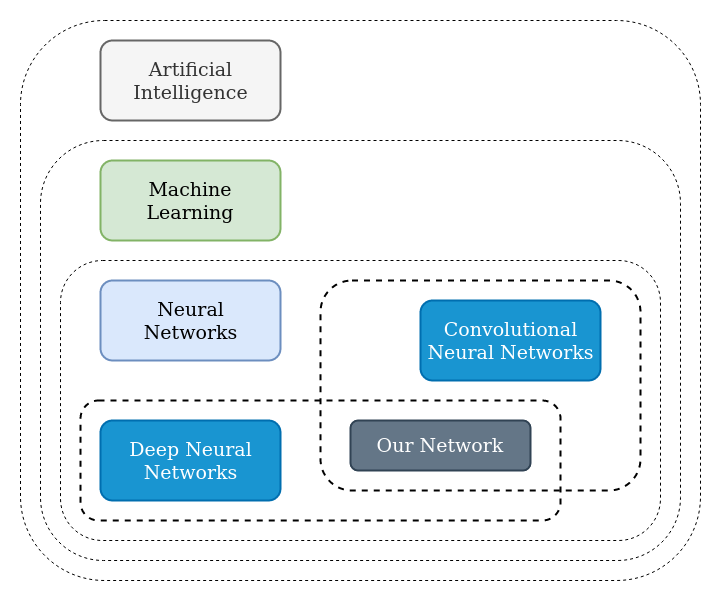
\includegraphics[width=0.7\textwidth]{Images/02_AI-ML-Scheme.png}
        \caption{The relationship between main fields}
        \label{fig:AI-ML-Scheme}
    \end{figure}
    
\subsection{Machine Learning} 
    Machine Learning (ML) is the 'field of study that gives computers the capability to learn without being explicitly programmed' \cite{Samuel1959SomeSI}. Technically, ML is an approach to data science and data analysis that involves adapting and building special computational models, which allow computer programs and algorithms to learn through set of repetetive steps and experience. It is based on many scientific areas such as: linear algebra, probability, graph theory or calculus and statistics. Machine Learning models are constructed and improved by dedicated algorithms which goal is to perform the best possible prediction or classification with most possible accuracy.
    
    There are various machine learning concepts and architectures, but these three elements are often included in most common designs:
    \begin{itemize}
        \item Model - the element which performs prediction
        \item Parameters - the factors used by the \textbf{model} to make decisions
        \item Learner - the part that adjusts the \textbf{parameters}
    \end{itemize}
    
    Machine Learning usually works by:
    \begin{itemize}
        \item gathering the data (where the quality of data determines the future quality of model), 
        \item processing the data to ensure consistence and relevance, 
        \item splitting the data to different sets (usually: training and test sets). 
        \item building the model using carefully chosen algorithm and techniques 
        \item evaluating and upgrading the model several times to reach the appropriate level of accuracy \cite{deepai}. 
    \end{itemize}
    
    ML model requires well-prepared data to work properly. In many approaches, the prepared batch of data usually includes label describing its type. It enables algorithm to distinguish the batches and learn about their specific features. 

    One way how we can classify the tasks that machine learning algorithms solve, is by the amount of labeled data and the computationally generated feedback. In the first type, some amount of properly labeled data is provided, and the model generates expected output. This paradigm is called \textbf{supervised learning}. 
    In another paradigm, no labeled data is provided, and no feedback is generated. This is  \textbf{unsupervised learning}. Lastly, the \textbf{reinforcement learning}, different than previous ones, take suitable action to maximize reward in a particular situation. The three main paradigms of Machine Learning are depicted in Figure \ref{fig:ML-paradigms}. \\
    \begin{figure}[ht]
        \centering
        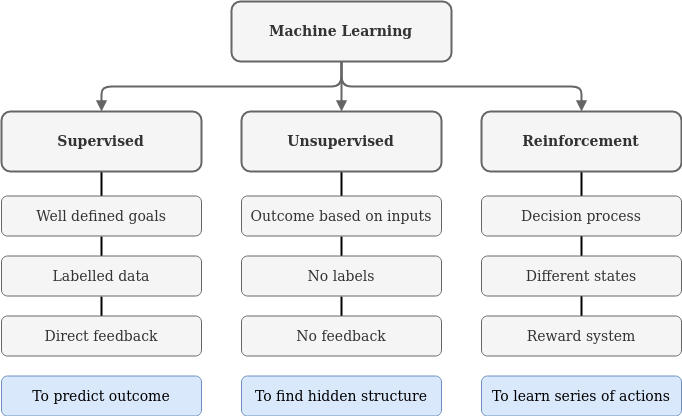
\includegraphics[width=0.7\textwidth]{Images/02_ml_paradigms.png}
        \caption{Machine Learning paradigms}
        \label{fig:ML-paradigms}
    \end{figure}

    There are a various applications to which ML methods can be implemented. The most popular ones \cite{MLgoogle} incl.: Natural Language Processing, Pattern Recognition, Classification Problems, Learning Associations and Image Processing. The last one is the main object of focus in this paper.

\newpage

\subsection{Neural Networks}
    \subsubsection{Overview}
    The neural network is a concept used for building a computer program that learns from provided data and which is loosely based on how the human brain works. It is a collection of artificial \textbf{neurons} which are connected to each other and forced to communicate. If a collection is asked to solve a problem, it attempts to do so, over and over again, each time strengthening the connections that lead to successful solution, and reduce those leading to the wrong one \cite{tfplayground}.
    
    More technically, neural networks are \textbf{weighted graphs}. They consist of an ordered set of layers consisting of neurons (also called nodes). The first layer of the neural network is called the \textbf{input layer}, and the last layer is called the \textbf{output layer}. The layers in-between are casually called \textbf{hidden layers}. Neurons belonging to one layer are connected to the neurons in the preceding and/or the previous layers. These connections are weighted edges. \\ 
    \begin{figure}[ht!]
        \centering
        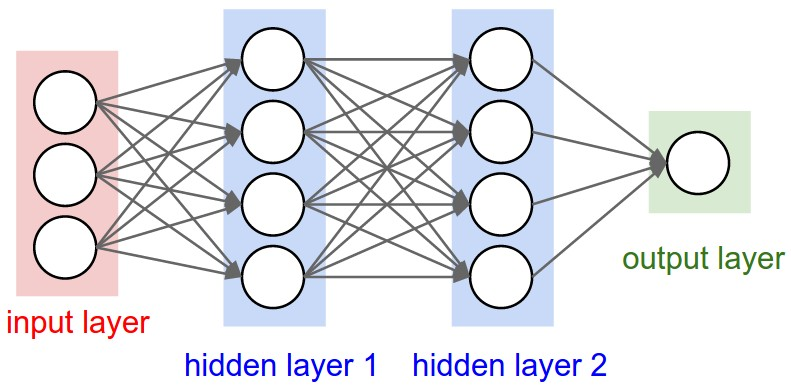
\includegraphics[width=0.7\textwidth]{Images/02_cnn_network_layers.jpeg}
        \caption{Neural network layers \cite{dlstanford}}
        \label{fig:02_cnn_network_layers}
    \end{figure}

    Given particular numerical input, each node produces an output value which is then calculated by the \textbf{activation function}. Output of this calculation is later passed to the next connected nodes, which are responsible for calculating next outputs. Thanks to this consecutive calculations, the network can calculate the final value in the output layer. This value is anticipated result of the process.
    
    \subsubsection{Deep Neural Networks}
    Deep neural network is generally defined as feed-forward network with numerous hidden layers. There is no official specification of number of layers needed to qualify neural network as a deep one. Usually having two or more hidden layers counts as deep. In contrast, a network with only a single hidden layer is described as "shallow" one \cite{Goodfellow-et-al-2016}.
    

\subsection{Convolutional Neural Networks}

    \subsubsection{Definition}
    \textbf{Convolution Neural Network} (mentioned later as CNN / Conv or ConvNet) is really important type of network. The \textbf{convolution} operation which originated CNN name, is a specific kind of linear operation. Convolutional networks are simply neural networks that use this convolution operation in place of general matrix multiplication. It may be used in one or more of their layers \cite{Goodfellow-et-al-2016}. CNN was designed to adapted the process of classifying images, but the same concept also fits other fields of machine learning processing such as classifying audio recording or videos. 
    Compared to the \textit{typical} feed-forward neural network with a similarly-sized layer, ConvNet might have fewer connections and parameters. It implies processing smaller batch of data and makes this type of networks easier to train, while its theoretically-best performance is going to be only slightly worse \cite{krizhevsky-imagenet}.

    \begin{figure}[ht!]
        \centering
        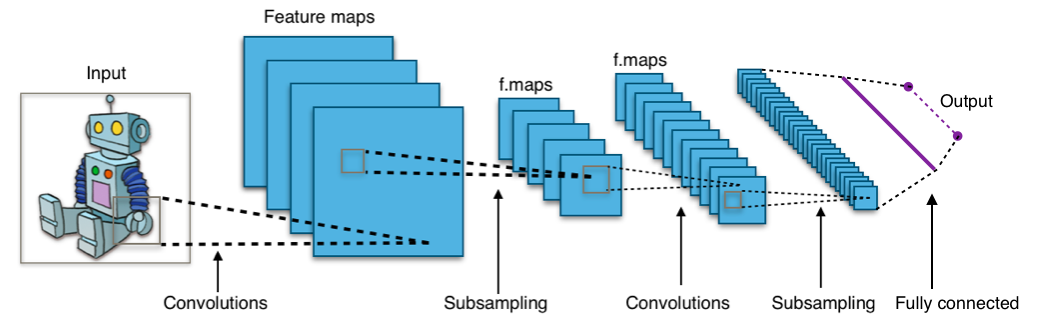
\includegraphics[width=0.5\textwidth]{Images/02_cnn_typical_wiki.png}
        \caption{Convolution with 3x3 filter \cite{wiki-cnn}}
        \label{fig:cnn-convolution-typical}
    \end{figure}
        
    \subsubsection{CNN Layers}
    The architecture of a CNN is designed to take advantage of the two-dimensional structure. Therefore it fits well to the concept of processing images which are generally stored as a two-dimensional arrays. CNN consists of one or more convolutional layers followed often by subsampling step (pooling), and then by one or more fully connected layers. \cite{dlstanford}. The most common ConvNet layers listed below are normally placed where the hidden layers are depicted on Figure \ref{fig:02_cnn_network_layers}. 
    \begin{itemize}
        \item The \textbf{convolution layer} is responsible for extracting features from the input. It computes a dot product between neuron weights and a small cropped region from input volume.
        \begin{figure}[ht!]
            \centering
            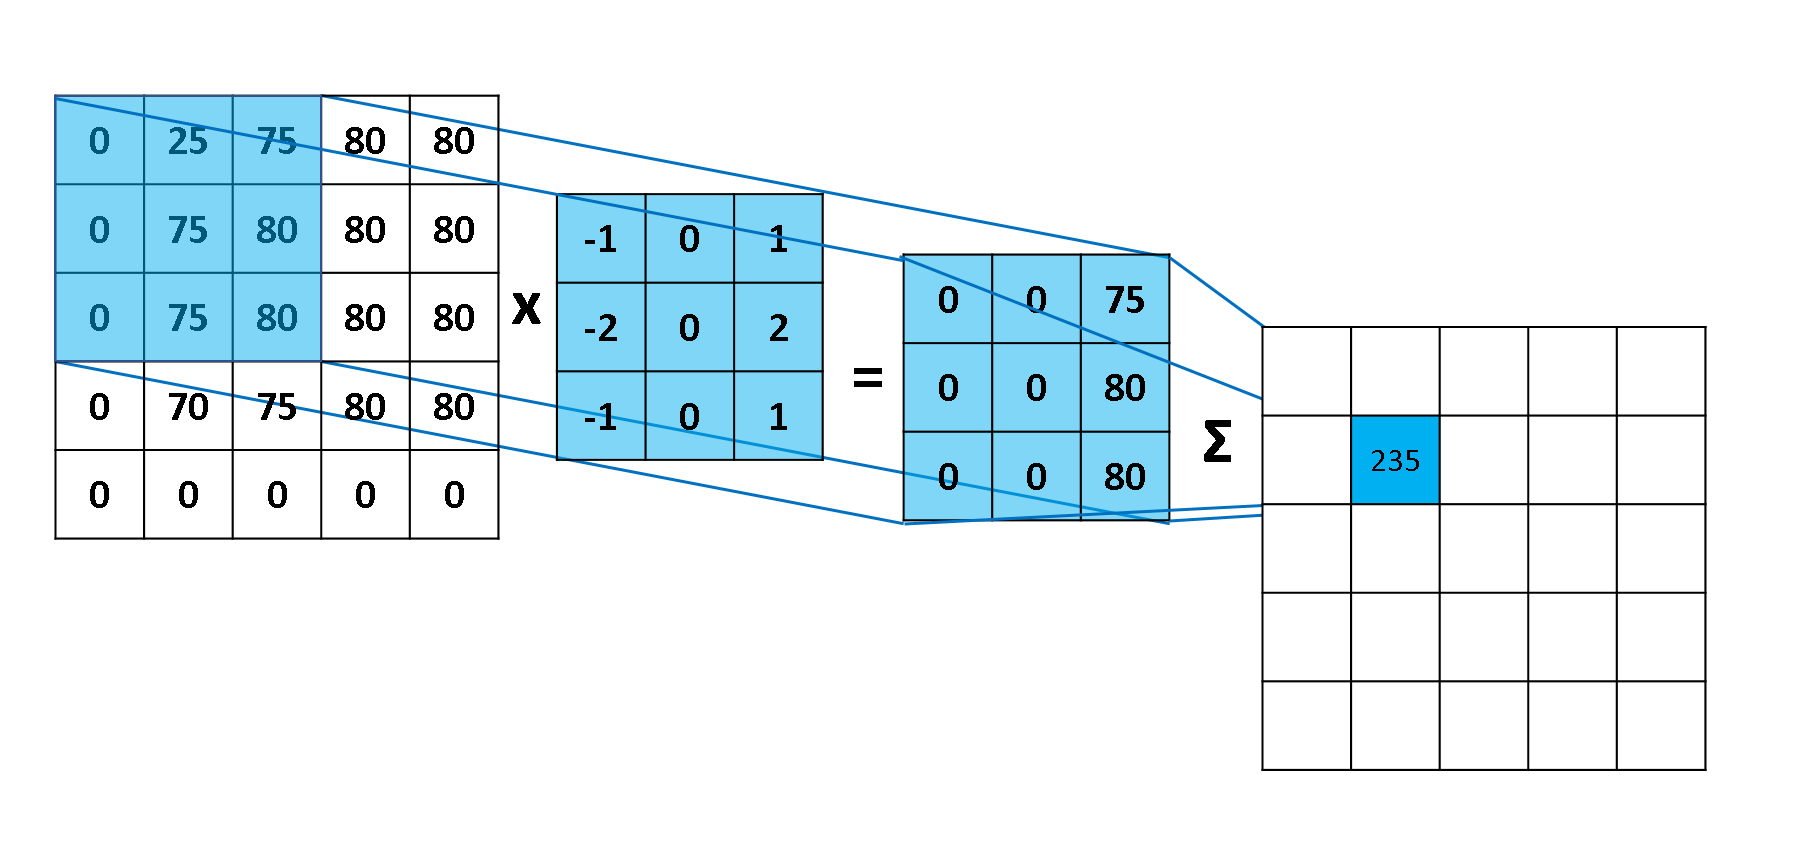
\includegraphics[width=0.5\textwidth]{Images/02_cnn_convolution.png}
            \caption{Convolution with 3x3 filter \cite{dlstanford}}
            \label{fig:cnn-convolution}
        \end{figure}
    
        \item The \textbf{pooling layer} reduces the spatial size of the feature maps. Sometimes, the input image consists of many pixels, so its processing is time-consuming, especially when the image is a part of huge dataset. In this case, the objective of the pooling layer is to reduce the spatial dimension of the input matrix. A pooling layer is applied after one or multiple convolution layers.
        \begin{figure}[ht!]
            \centering
            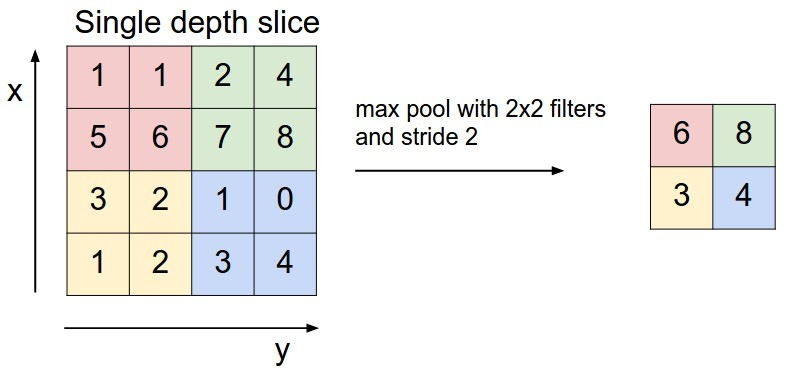
\includegraphics[width=0.5\textwidth]{Images/02_cnn_pooling.jpeg}
            \caption{Process of max-pooling \cite{dlstanford}}
            \label{fig:cnn-pooling}
        \end{figure}
        
        \item The  \textbf{fully connected layer} - performs the high-level reasoning and produces the final output. Neurons in a fully connected layer have connections to \textbf{all} neurons in the previous layer.
        \begin{figure}[ht!]
            \centering
            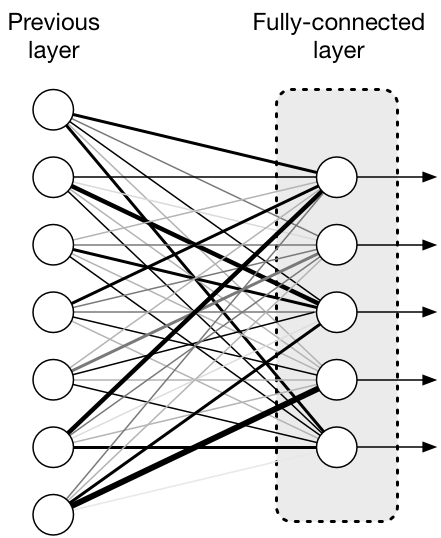
\includegraphics[width=0.25\textwidth]{Images/02_cnn_fully_connected.png}
            \caption{Fully-connected layer \cite{medium-teco}}
            \label{fig:cnn-fully-connected}
        \end{figure}
    \end{itemize}


    \subsubsection{Loss}
    The function that allows solutions to be ranked and compared is necessary for determining if the result of operations performed in a neural network is correct (or not). It is called \textbf{loss function} and reduces all the various good and bad aspects of a possibly complex system down to a single number (or vector of numbers), which evaluates the candidate solution \cite{neuralsmithingbook}. 
    
    \subsubsection{Activation}
    The activation function is attached to each neuron in CNN. It is used to decide whether particular neuron should be activated or not ,based on whether neuron input is relevant for the model prediction. Activation functions also helps to normalize the output of each neuron to some range. The standard range is [0,1] or [-1,1] which prevents the output values to grow rapidly and cause computational problems \cite{missinglink}. 

    Since activation is calculated for thousands or even millions of neurons for each data sample, it has to be computationally efficient. The one of the most popular activation function is \textbf{Rectified Linear Unit (ReLU)}. It applies an element-wise function, such as the max(0,x) - thresholding at zero - to either activate or deactivate each single neuron.

    \subsubsection{Backpropagation}
    Backpropagation is an algorithm commonly used to \textbf{train} neural networks. When the neural network is initialized, weights are set randomly or randomly-like. The input is loaded and then passed through the network, and it provides an output for each one neuron, given the initial weights. Backpropagation for a convolution operation (for both the data and the weights) is also a convolution. It helps to adjust the weights of the neurons so that the result comes closer and closer to the known true result. 

% \newpage

\subsection{ResNet}
    \textbf{Residual Network} - is an another type of neural network that can be used to perform many machine learning tasks. ResNet was introduced in paper "Deep Residual Learning for Image Recognition" \cite{ResNet2015}.
    
    \subsubsection{Background}
    Since first successful approaches to construct deep neural network which achieves great accuracy prediction with high efficiency, researchers was trying to compose deeper and deeper network. Each next popular network consists of more and more convolution layers stacked together - AlexNet (5), VGG (19) and then GoogleNet (22). \cite{tds-resnet}

    However, it turns out that deeper networks experienced the \textbf{vanishing gradient problem}. Due to the repeated multiplication in all layers, gradient becomes really small value, close to the infinity. Network having this problem is harder to train and its performance might degrade. Therefore, scientist start seeking a solution, how to reduce or to remove vanishing gradient problem. The best idea was presented in 2015, called ResNet \cite{ResNet2015}

    \subsubsection{Core concept}
    Author \cite{ResNet2015} proposed the new key element implemented in NN - Residual Block (\ref{fig:resnet-compared}. 
    It has a direct connection which skips some layers in between (number of skipped layers varies in different models). This connection is called \textit{skip connection} and is the core of residual blocks. It allows alternate shortcut path for the gradient to flow through. It also helps by allowing the model to learn the identity functions, which ensures that the higher layer will perform at least as good as the lower layer.
    
    \begin{figure}[H]
        \centering
        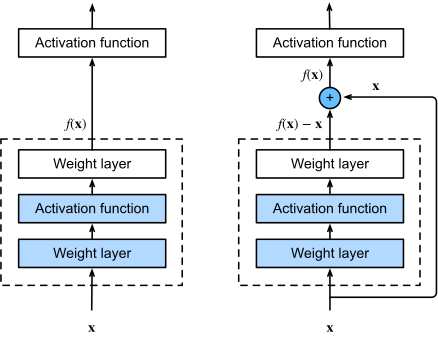
\includegraphics[width=0.4\textwidth]{Images/02_resnet_compared.png}
        \caption{Residual block (right) compared to standard block (left) \cite{d2l-ai}}
        \label{fig:resnet-compared}
    \end{figure}

    \subsubsection{Architecture}
    Skipping connections makes possible to create very deep neural networks with more than 1000 layers. But the most common versions of ResNet are ResNet34 and ResNet50 with number of layers indicated in the name. In this paper we focus on ResNet34, using it for image classification. This architecture won several awards p.e. on ILSVRC and COCO contests, dethroning the VGG architecture. The comparison of VGG-19 architecture, 34-layers network and 34-layers ResNet is presented on \ref{fig:resnet34} and will be referenced further in this paper. 
    
    \begin{figure}[ht!]
        \centering
        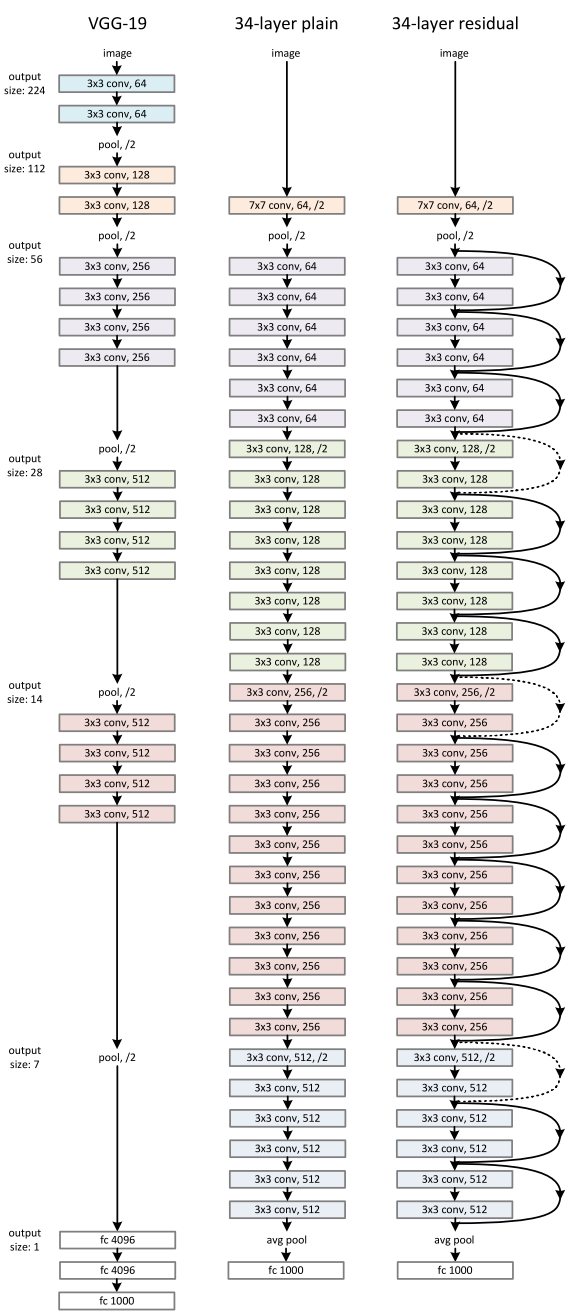
\includegraphics[width=0.6\textwidth]{Images/02_resnet34.png}
        \caption{ResNet34 architecture (right) compared with network without residual connections (middle) and classic VGG-19 (left) \cite{tds-resnet}}
        \label{fig:resnet34}
    \end{figure}

\newpage

\subsection{MobileNet}
    MobileNet convolutional neural network model (open-sourced by Google) designed to be used in mobile applications first introduced in 2017 \cite{MobileNet2017}. It significantly reduces the number of parameters when compared to the network with regular convolutions with the same depth in the nets. This results in the most important MobileNet feature - being lightweight deep neural network suitable for mobiles.
    
    \subsubsection{Core concepts}
    Several factors made MobileNet great solution for many use cases:
    \begin{itemize}
        \item Depthwise separable convolution - a depthwise convolution followed by a pointwise convolution. There are two different variations of standard convolution idea - the first one is a map of a single convolution on each input channel separately. And the next one is simple 1x1 convolution. Stacking them together reduces computation around 8 times \cite{MobileNet2017}, but with only small reduction in accuracy.
            \begin{figure}[H]
                \centering
                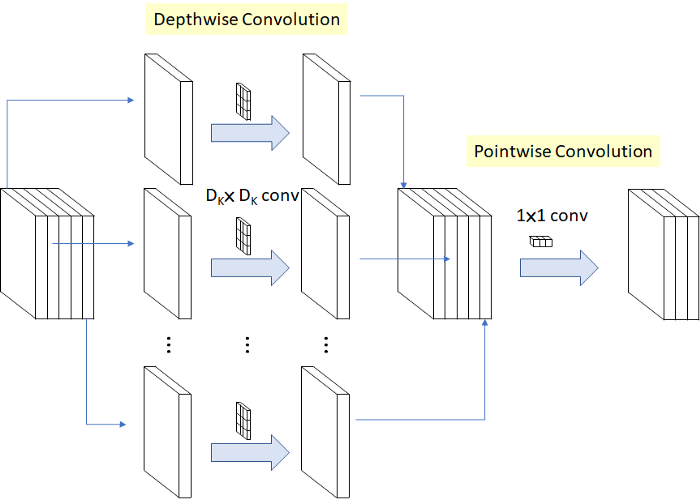
\includegraphics[width=0.5\textwidth]{Images/02_mobilenet_deepwise.png}
                \caption{Depthwise Separable Convolution \cite{MobileNet2017}}
                \label{fig:mobilenet-dsc}
            \end{figure}
        
        \item Batch Normalization - both Batch Normalization and ReLU are applied after each convolution which also reduces the final number of network parameters
        
        \item Multipliers - Width Multiplier \textit{alpha} is introduced to control the number of channels or channel depth and the Resolution Multiplier \textit{ro} is introduced to control the input image resolution of the network \cite{tds-mobilenet}
    
    \end{itemize}
    
    \subsubsection{Comparision}
        MobileNet does not attempt to beat the other neural network models in terms of accuracy, but instead, focuses on reducing the number of parameters and the \textit{weight} of the model. It can be seen on \ref{fig:mobilenet-comp}, where authors of MobileNet compare it to other popular architectures.
            \begin{figure}[H]
                \centering
                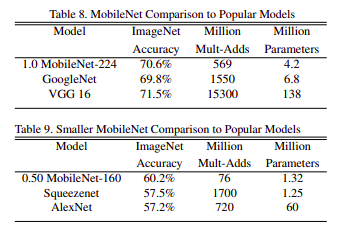
\includegraphics[width=0.5\textwidth]{Images/02_mobilenet-comparision.png}
                \caption{MobileNet comparison to popular models \cite{MobileNet2017}}
                \label{fig:mobilenet-comp}
            \end{figure}
    
    
    
% \newpage

\subsection{Computer Vision}
    Computer Vision (CV) is a field of computer science, that seeks to understand the images and videos. Inspect how they are stored, how can they can be manipulated and how can we effectively retrieve data from them. It tries to replicate the our natural vision system and enable computers to 'see and process' the same way humans do. Computer Vision plays a major role in photo correction applications and art generation, but also in self-driving vehicles or robotics \cite{towardsdatascience}.
    
    Due to the growing popularity of AI and recent innovations in the field of Deep Learning, CV is developing rapidly and is able to achieve better results in almost all areas of common research. In several tasks, it even can surpass humans capabilities such as object detection or image labeling. 

    \subsubsection{Image classification}
    Image classification refers to the task of assigning a label to an image. Typically, Image Classification refers to images in which only one object appears and is analyzed. In contrast, object detection involves both classification and localization tasks, and is used to analyze more realistic cases in which multiple objects may exist in an image. This paper focuses on the first task, which is extracting and classyfing only one object from the image. \cite{googledev-images}
    
    As mentioned before, image classification is a supervised learning problem. We define a set of target classes which are objects to identify in images, and try to train a neural network model to recognize them using labeled example photos. Early computer vision models relied on raw pixel data as the input to the model which causes many problems when images have poor quality or are taken in different environment. Future approach uses CNN to carefully analyze and process each part of an image, as shown on \ref{fig:image-classification}. 
    
    \begin{figure}[H]
        \centering
        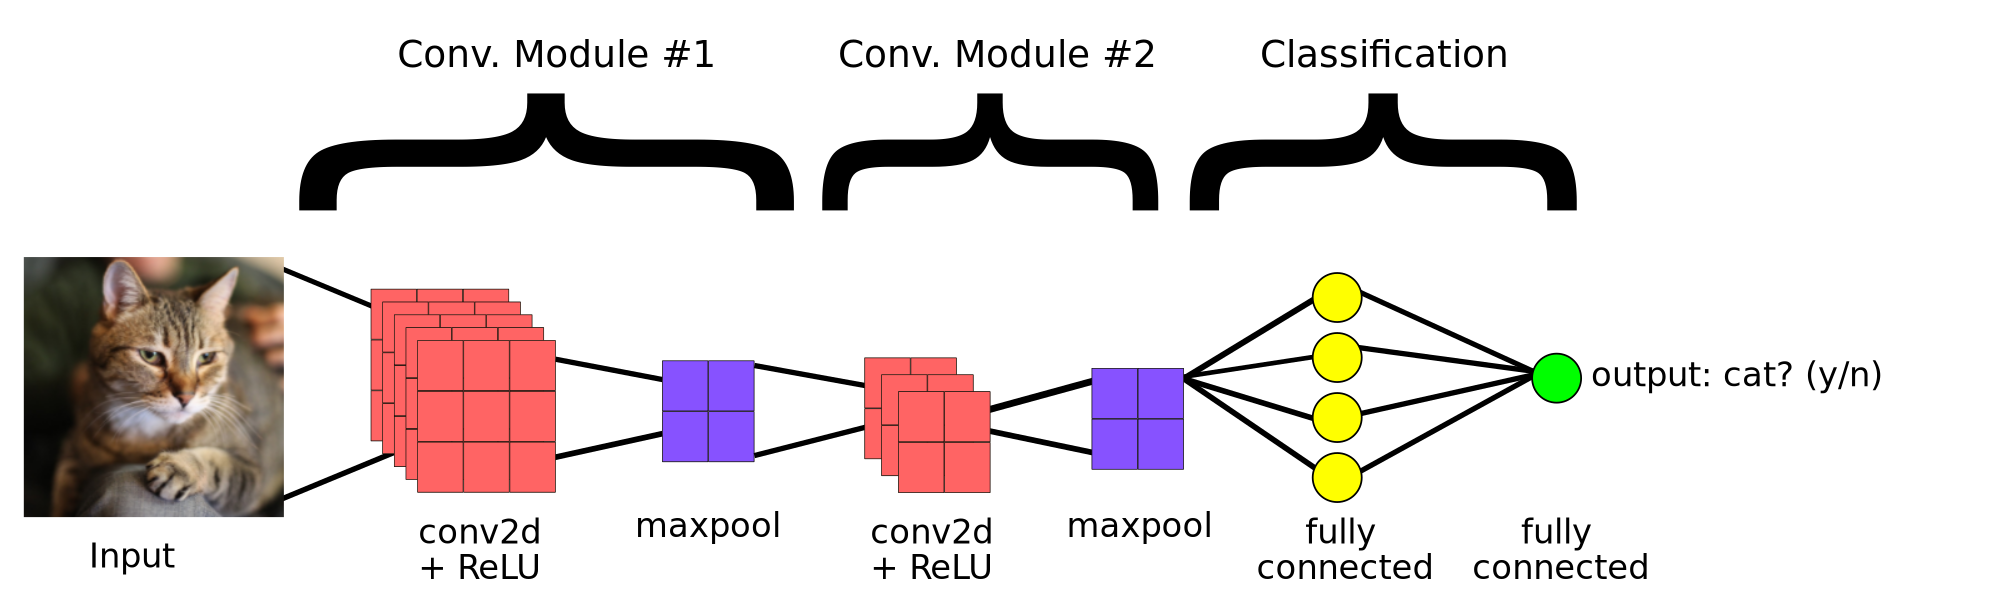
\includegraphics[width=0.8\textwidth]{Images/02_imclass_google.png}
        \caption{Example of image classification using CNN from Google Developer Practicum \cite{googledev-images}}
        \label{fig:image-classification}
    \end{figure}

\newpage

\subsection{State of the art}
    \subsubsection{Tree recognition}
    \begin{itemize}
        \item \textbf{Texture features} \\
        Early approaches to the tree recognition were not using deep networks. In 2006 the article of \cite{Huang2006} was published and described extracting texture features
        based on Gabor wavelet using a radial basis probabilistic network as the classifier. Authors obtained accuracy around 80\%, but on relatively small dataset of 300 tree images. 
        
        It works by decomposing an image into 6 sub-bands using the 7-9 'biorthogonal Debauches wavelet' transform. Each sub-band was fed to the directional filter banks stage. After that, the mean and stdev of the image output are computed. The obtained feature vectors are fed up into radial basis probabilistic network which classify the image.
        
        Even though the final results are not terrific comparing to current standards, we must remember that it was developed in \textit{before-deep-learning} era. This technique is highly sophisticated and thus worth to mention.


        \item \textbf{Lidar scan} \\
        When popularity of deep networks start growing, much more papers referring to tree recognition were released. They are differ in terms of source images used for classification. One interesting technique was presented in 2017 by \cite{Lidar2017} using LIDAR scan method. Terrestrial Lidar scan is commonly used for detailed documentation in the field of forest inventory investigation. It is able to obtain high resolution point cloud (resolution of 5 mm at a 10 m distance) in the shady forest area. Images can be later converted to depth image of size 256x256.
        
        In this case larger dataset was used containing 35 000 transformed and cropped Lidar scans. Classification was performed by network based on a standard AlexNet \cite{krizhevsky-imagenet} and the accuracy of ~90\% was reached.
        
        Unfortunately, the authors focused only on Japanese cedar and cypress, what undoubtedly makes the problem less challenging and the model less reusable.

        \begin{figure}[H]
            \centering
            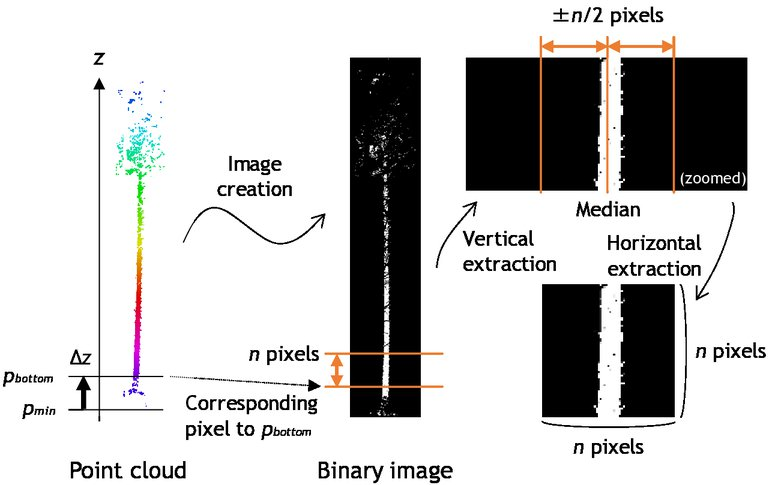
\includegraphics[width=0.7\textwidth]{Images/stateofart/03_art_lidar.jpg}
            \caption{Lidar scan transformed to depth images \cite{Lidar2017}}
            \label{fig:03_art_lidar}
        \end{figure}
        
        
        \item \textbf{Wood core scan} \\
        Another paper \cite{Fabijanska2021} tackles the problem of automatic tree species identification from different source - scanned photos of wood cores. 
        
        The generic architecture was used to solve this task - a convolutional neural network with residual connections. The model was applied to subsequent image patches following the sliding window strategy to recognize a patch central pixel’s membership. Majority voting was used to select the tree species. Once again, the project was based on small dataset - consisting of only 312 wood core images. The proposed model correctly recognized species of almost 93\% the wood image patches and 98.7\% of wood core images.
        
        Although the results are promising and the authors are on a way to extend the research in this field, one has to remember that gathering data to process through this model is complicated task. Wood core images have to be carefully extracted and scanned in high quality, what makes this approach impossible to implement in user-friendly mobile technologies. 
        
        \begin{figure}[H]
            \centering
            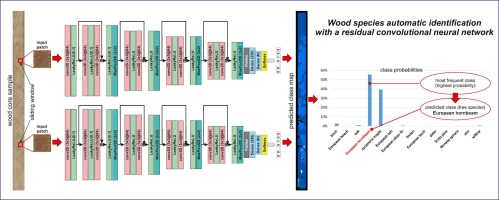
\includegraphics[width=0.7\textwidth]{Images/stateofart/03_art_dendro.jpg}
            \caption{Simplified flow of recognition system developed by \cite{Fabijanska2021}}
            \label{fig:03_art_dendro}
        \end{figure}
        
        \item \textbf{Aerial} \\
         Significant amount of first works for tree species classification mainly focused on aerial or satellite images, rather than using ground-based sensor data. Plenty of articles were based on technique called photo-interpretation. The good example is paper \textit{Tree species identification on large-scale aerial photographs in a tropical rain forest} \cite{VALERIE200651}. Authors were analyzing large photos of French Guiana forests trying to identify plant species. For training they use sub-images marked by botanical specialist. 2188 trees of 130 species were flagged. They develop a segmentation method based on colour, texture and shape criteria, and work within an image processing environment that automatically designs recognition operators at several spatial resolutions.  The average accuracy was pretty high and reached the level of 87\%. 
         
         Later approaches, using deep learning overcome this results, but still we have to acknowledge the amount of work done in this area without deep learning. 
         
         The recent publications, such as \textit{Classification of the tree for aerial image using a deep convolution neural network and visual feature clustering} \cite{Lin2020} obtains excellent results providing great tools for aerial photo analysis.
         
         Using supervised machine learning methods for treed areas classification and combining them with unsupervised color clustering allow achieving optimum outcome.
         The authors use YOLO model to obtain tree features and location information. Then Flood Fill and K-means algorithms were used for tree classification experiments: measuring precision, accuracy and recall rate. They can distinguish in shape, illumination, and angle of tree species, as well as color differences affecting classification results. 
         
         Despite the fact that these kind of images cannot be easily captured and provided to mobile application, they serve another major purpose. They can support analyze and understanding of land use and land cover changes in the era of over-exploitation and accelerated destruction of rural and natural environments.

            \begin{figure}[H]
                \centering
                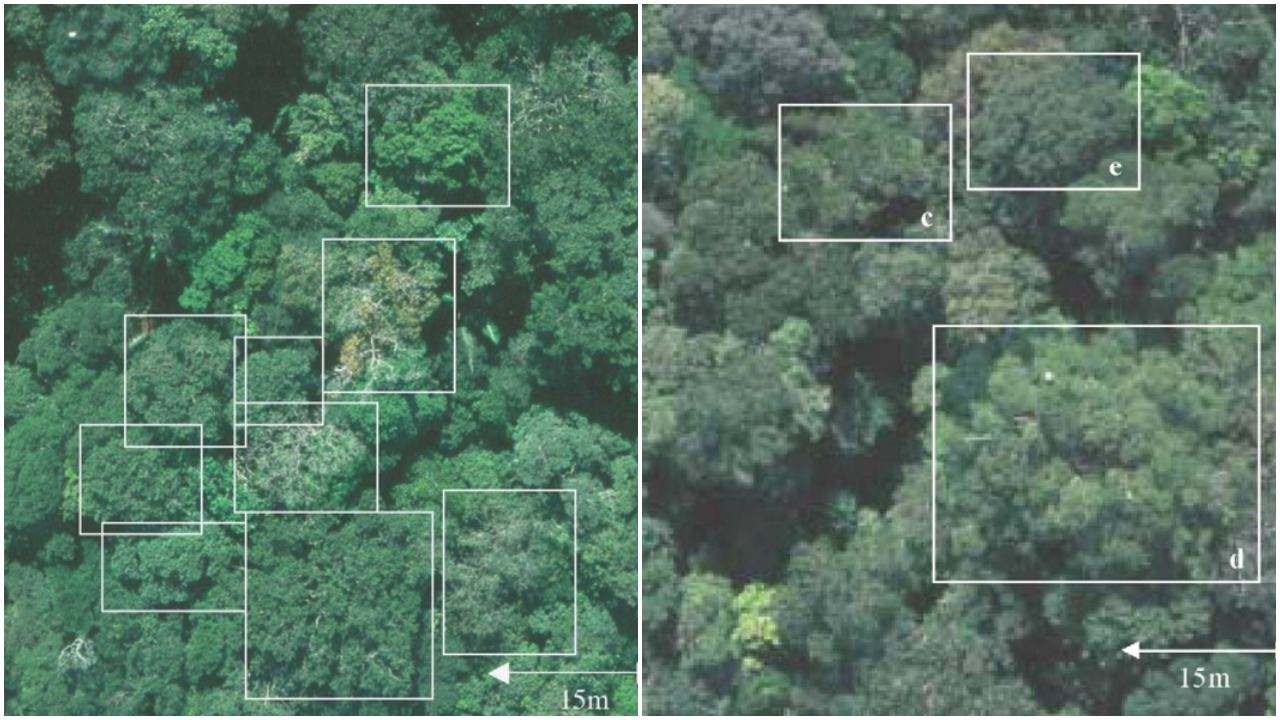
\includegraphics[width=0.7\textwidth]{Images/stateofart/03_art_aerial_combined.jpg}
                \caption{Aerial forest photographs \cite{VALERIE200651}}
                \label{fig:03_art_aerial_combined}
            \end{figure}
        
        \item \textbf{Bark}
        new sublist
        - from article: https://arxiv.org/pdf/1803.00949.pdf
        - main work: treebark
        
    \end{itemize}
    
    \subsubsection{Plant recognition}
    \begin{itemize}
    
        \item \textbf{LifeCLEF / PlantCLEF} \\
        The LifeCLEF \cite{clef} plant identification challenge is an important milestone towards automated plant identification systems working at the scale of continental floras with 10.000 plant species living mainly in Europe and North America illustrated by a total of over 1mln images. 
        
        The goal is to retrieve the correct plant species among the top results of a ranked list of species returned by the evaluated system. Queries are defined as s as plant observations, meaning a set of 1 to 5 images depicting the same individual plant observed by the same person the same day.
        
        A part of PlantCLEF dataset is be provided as training data whereas the remaining part is used later as test data.
    
        \item \textbf{Plant images from noisy web data} \\
        The paper \cite{CLEF2017} created as a result of LifeCLEF 2017 plant challenge presents another examples of novel approaches to plant recognition.
        
        Training dataset was collected through the web and containing a lot of labelling errors what is in opposite to standard smaller but trusted training dataset checked by experts. 
        
        The main conclusion of this paper was that CNN architectures appear to be 
        effective in the presence of noise in the training set. All networks from challenge, trained on the noisy dataset, did significantly outperform the same models trained on the less noisy (trusted) data. In every case, it was more profitable to use the noisy training data. Authors of the paper conclude that diversity in the training data is a key factor to improve the generalization ability of deep learning.
        
        This is an obvious suggestion to use convolutional neural networks and huge datasets in attempt to successfully classify plant images.

        \item \textbf{Wildflowers Project} \\
        Accurate identification of wildflowers is a task with relevance to both recreation and environmental management. The aim of \textit{wildflowers.com} project (based on paper introduced by \cite{Sulc2016}) was to develop a model that could take advantage of metadata provided by users of a mobile app while photographing wildflowers in order to provide more accurate classifications. This objective seems pretty similar to objective of my project, therefore it is worth to mention the outcome of WildFlowers \cite{wildflower}. 
        
        Author decided to collect photographs of local wildflowers using his iPhone and a point and shoot camera. Yet again the dataset is small and contains only 651 images representing 11 wildflower species. To reduce overfitting images were resized (to 256x256) and cropped (to 224x224) and then re-generated using Keras random data augmentations.
        
        The core of the project is ResNet50 \cite{ResNet2015} - neural network already trained to detect basic features in objects. By adding fully connected layers specific to the wildflower data, author fine-tuned this network to apply its understanding of basic objects to identify features that distinguish our flower classes.
        Final model accuracy after testing on 306 images was 97\% what makes it interesting source of inspiration for similar project.
        
    \end{itemize}
    
    \subsubsection{Leaf recognition}
    

\biblio % Needed for referencing to working when compiling individual subfiles - Do not remove
\end{document}
